\section{引言}

\begin{figure}[tb]
  \centering
  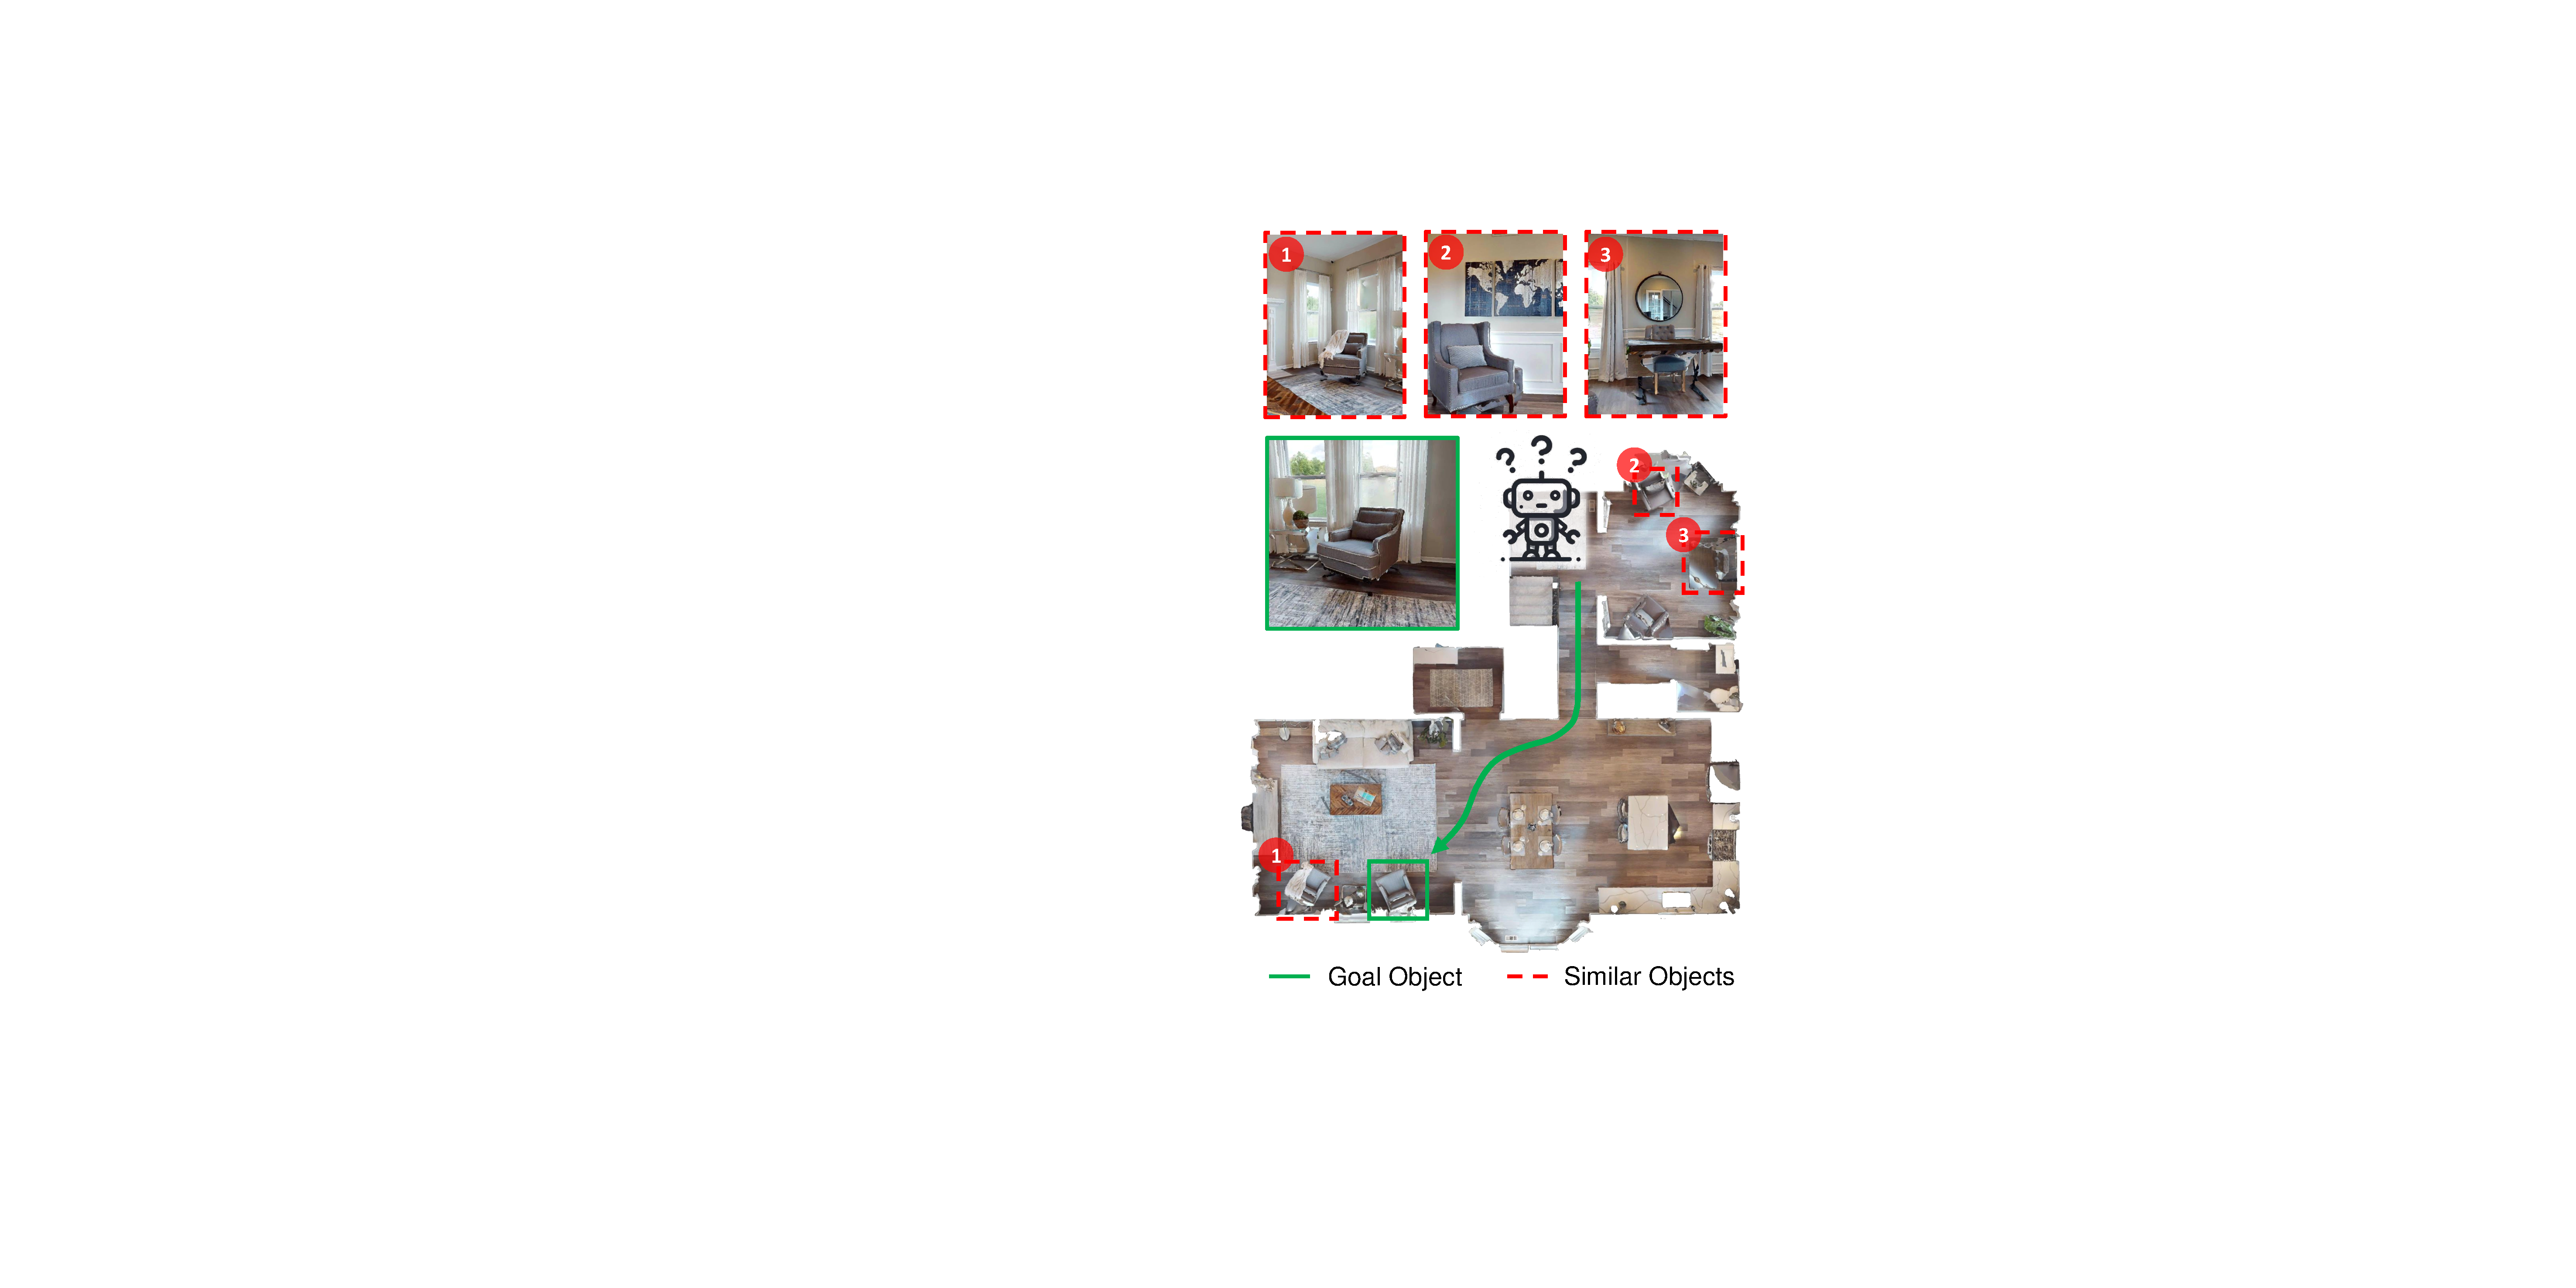
\includegraphics[width=0.9\linewidth]{pics/intro.pdf}
  \caption{实例图像目标导航(IIN)示意图。该任务要求智能体导航至目标图像所描绘的物体实例，同时将其与其他视觉相似的实例区分开来。
  }
  \vspace{-16pt}
  \label{fig:intro}
\end{figure}


\IEEEPARstart{具}{身}视觉导航是一个新兴的计算机视觉问题，它要求智能体利用视觉感知主动与世界交互并完成导航任务\cite{cheng2022learning, krantz2022sim, zhang2022generative, lin2022multimodal, qiao2023hop+, cai2021pose, lin2021adversarial, an2024etpnav, wu2023human, wang2020vision, wang2023learning, wang2022towards}。近年来，随着大规模真实感三维场景数据集\cite{xia2018gibson, yadav2023habitat, chang2017matterport3d}和快速具身导航模拟器\cite{szot2022habitat, kolve2017ai2, savva2019habitat}的出现，具身视觉导航领域取得了长足进步。这些进展使研究人员能够在高度模拟真实世界条件的受控环境中开发和测试导航算法。

在具身视觉导航中，一个核心问题是"我们如何描述目标对象"。一种常见的任务设定是向智能体提供自然语言指令，例如"检查我的笔记本电脑是否在椅子上"。然而，当房间里有多把椅子时，这种设定就会产生歧义。为解决这一挑战，Krantz等人\cite{krantz2022instancespecific}提出了实例图像目标导航(IIN)\cite{krantz2023navigating, bono2023endtoend, lei2024instanceaware}。在IIN任务中，智能体被提供一张特定物体的图像，其目标是在最短时间预算内导航至该特定物体。如\Cref{fig:intro}所示，目标图像无需与导航智能体的传感器规格或身体形态相匹配。为完成该任务，智能体需要在不同视角下识别目标物体，并忽略潜在的干扰物。这是一项极具挑战性的任务，因为它涉及语义推理、几何理解和实例感知匹配。

为解决上述问题，现有方法\cite{chaplot2020learning, chaplot2020object, krantz2023navigating, ramakrishnan2022poni, al2022zero, ma2022end, lei2024instanceaware}引入了二维语义鸟瞰图(BEV)地图来解决该问题。这些精心设计的显式地图表示具有内存高效的特点，能够存储二维几何和语义等关键信息，并可直接用于计算智能体的后续动作。然而，这种简单的二维BEV地图表示缺乏保留环境三维几何信息的能力，因此无法有效处理跨楼层导航场景。此外，BEV地图无法保留场景中的实例感知特征，而这些特征对于区分同一类别的多个物体或需要细粒度物体交互的任务至关重要。

% 这引出了一个问题：我们能否为具身智能体构建一种统一的地图表示来解决视觉导航问题？

为克服BEV地图的局限性，我们提出了一种全新的高斯泼溅导航框架，即GaussNav，用于解决IIN任务。我们的GaussNav框架受到三维视觉技术最新进展的启发，包括神经辐射场(NeRF)\cite{mildenhall2020nerf}和三维高斯泼溅(3DGS)\cite{kerbl3Dgaussians}。这些技术在新视角合成(NVS)和三维场景理解方面取得了重大突破。尽管这些技术最初并非为导航任务开发，但它们在该领域具有巨大的应用潜力。为此，我们提出了语义高斯地图表示，它整合了几何、语义和实例感知特征的表示，可直接用于视觉导航。

我们的GaussNav框架包含三个阶段：前沿探索、语义高斯构建和高斯导航。
首先，智能体通过前沿探索收集未知环境的观测数据。
其次，利用收集到的观测数据构建语义高斯。通过语义分割算法\cite{he2017mask, wang2023internimage}，我们为每个高斯分配语义标签。然后根据语义标签和三维位置对高斯进行聚类，将场景中的物体分割为不同语义类别下的不同实例。这种表示不仅能够保留场景的三维几何和每个高斯的语义标签，还能保留场景的纹理细节，从而支持新视角合成。
最后，我们为物体实例渲染描述性图像，将其与目标图像进行匹配，从而有效定位目标物体。在确定预测目标物体的位置后，我们可以高效地将语义高斯转换为栅格地图，并使用路径规划算法完成导航。

据我们所知，我们是首次将三维高斯泼溅(3DGS)\cite{kerbl3Dgaussians}引入具身视觉导航领域的研究者。在本工作中，我们统一了视觉导航中几何、语义和实例感知特征的地图表示。我们的框架能够通过单张目标图像输入直接定位目标物体，并引导智能体导航至目标，无需额外的探索或验证步骤\cite{lei2024instanceaware}。我们的框架设计有助于实现高效且有效的视觉导航。我们在有效性和效率两个方面对所提方法进行了评估，并在极具挑战性的Habitat-Matterport 3D数据集(HM3D)\cite{yadav2023habitat}上创下了新的最优性能记录。